% Chapter 1
\chapter{پروتکل \lr{Openflow}}
با توجه به توضیحات گفته شده در مقدمه، ارتباط کنترل کننده‌ها با بخش هدایت داده از طریق ارتباط جنوبی\LTRfootnote{Southbound Interface} برقرار می‌گردد. برای برقراری این ارتباط پروتکل‌های مختلفی وجود دارد که \lr{Openflow (OF)} یکی از پر کاربردترین آن‌ها است.

\section{\lr{Openflow}}
پروتکل \lr{(Openflow)} که توسط بنیاد آزاد و بدون منفعت \lr{Open Networking Foundation (ONF)} استاندارد سازی و توسعه داده می‌شود، یکی از مهم ترین پروتکل‌های موجود برای ارتباط کنترل کننده و سوئیچ‌ها بوده که از همان ابتدای پیداش تحولات شبکه و حرکت به سمت تعریف بر اساس نرم‌افزار، به عنوان نمادی برای جداسازی بخش تصمیم گیری و بخش هدایت مورد توجه قرار گرفته است.\\
در طی سال‌های متمادی پس از عرضه و استاندارد سازی این پروتکل توسط \lr{ONF}، تغییرات و به روز رسانی‌های بسیاری را تجربه کرده تا بتواند پاسخگوی نیاز‌های به‌روز شبکه باشد و امروز که در حال تهیه این گزارش هستیم نسخه \lr{OF1.5.1} آن توسط \lr{ONF} تهیه و منتشر شده است. بسیاری از کمپانی‌های تولید کننده تجهیزات \lr{SDN} و کنترل کننده‌ها همچنان از نسخه‌های قدیمی تر استفاده می‌کنند اما در آینده نزدیک با پیشرفت سازگاری تجهیزات و کنترل کننده‌ها استفاده از نسخه‌های جدیدتر به صورت گسترده ممکن خواهد شد.

\section{اجزاء تشکیل دهنده سوئیچ \lr{Openflow}}

\begin{figure}
	\centering
	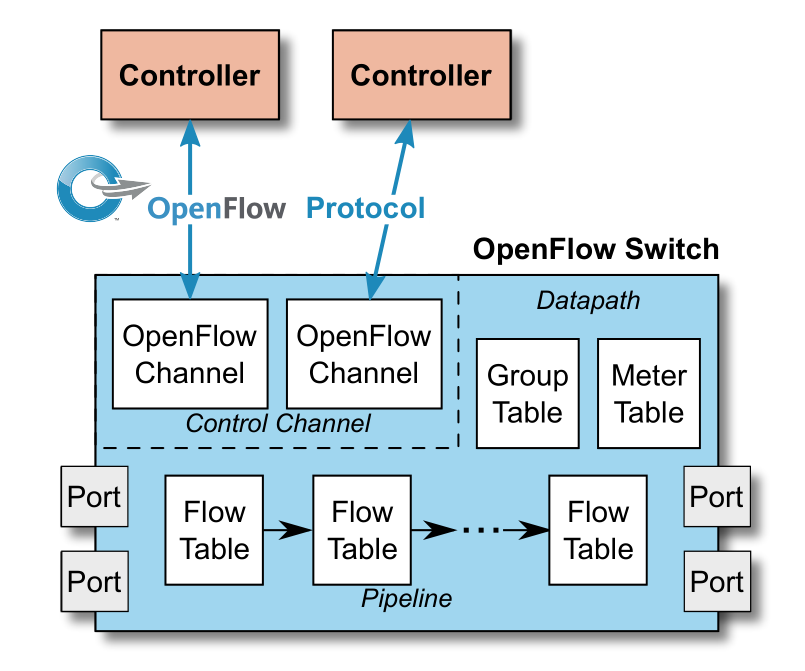
\includegraphics[scale=0.4]{imgs/of_comp.png}
	\caption{نمایی کلی از اجزاء اصلی یک سوئیچ \lr{Openflow}}
	\label{fig4}
\end{figure}

با توجه به شکل \ref{fig4} یک سوئیچ \lr{Openflow} از اجزاء مختلفی تشکیل شده است که در ادامه به معرفی هر بخش و کاربرد‌های آن می‌پردازیم \cite{spec}.

\subsection{\lr{Openflow Channel}}
کانال \lr{Openflow} بستری است که اتصال بین سوئیچ منطقی را با کنترل کننده فراهم می‌کند. از طریق این بستر، کنترل کننده قادر به پیکربندی و مدیریت سوئیچ، دریافت رخداد‌ها از سوئیچ و ارسال بسته‌ها خارج از سوئیچ می‌باشد. کانال کنترلی یک سوئیچ ممکن است از یک ارتباط کانال \lr{Openflow} به یک کنترل کننده پشتیبانی کند و یا قادر به پشتیبانی از ارتباط چندگانه کانال \lr{Openflow} به چند کنترل کننده باشد.\\
نوع ارتباط بین کنترل کننده و لایه هدایت داده به نحوه پیاده سازی آن بستگی دارد اما قالب داده‌های رد و بدل شده بین این دو باید طبق استاندارد \lr{Openflow} باشد. کانال \lr{Openflow} می‌تواند بر بستر رمزنگاری شده \lr{TLS} انجام گیرد یا به صورت مستقیم از \lr{TCP} استفاده کند. پیش‌فرض درگاه ارتباطی برای این اتصال در نسخه‌های اولیه \lr{TCP:6633} یا \lr{TCP:976} بوده است اما با عرضه نسخه \lr{OF1.4} این درگاه توسط \lr{IANA} به \lr{TCP:6653} تغییر کرد.
\pagebreak

در بستر ارتباط فوق الذکر، جا‌به‌جایی داده‌ها بین کنترل کننده و سوئیچ به دو دسته زیر تقسیم می‌گردد:
\begin{itemize}
	\item
کنترل کننده به سوئیچ: این پیام‌ها توسط کنترل کننده ارسال شده و ممکن است نیاز به جواب از سمت سوئیچ را داشته باشند. لیست انواع مختلف این نوع پیام به شرح زیر است:
	\begin{itemize}[noitemsep,topsep=0pt,parsep=0pt,partopsep=0pt]
		\item \lr{Features}
		\item \lr{Configuration}
		\item \lr{Modify-State}
		\item \lr{Read-State}
		\item \lr{Packet-out}
		\item \lr{Barrier}
		\item \lr{Role-Request}
		\item \lr{Asynchronous-Configuration}
	\end{itemize}
	\item
غیر‌همزمان: این پیام‌ها توسط سوئیچ و بدون فرمان از سمت کنترل کننده ارسال می‌شوند که بیانگر تغییر وضعیت سوئیچ یا رسیدن بسته می‌باشد. لیست انواع مختلف این نوع پیام به شرح زیر است:
	\begin{itemize}[noitemsep,topsep=0pt,parsep=0pt,partopsep=0pt]
		\item \lr{Packet-in}
		\item \lr{Flow-Removed}
		\item \lr{Port-status}
		\item \lr{Role-status}
		\item \lr{Controller-Status}
		\item \lr{Flow-monitor}
	\end{itemize}
\end{itemize}

\subsection{\lr{Openflow Ports}}
در یک سوئیچ \lr{Openflow} پکت‌ها از طریق درگاه‌های ورودی\LTRfootnote{Ingress Ports} به خط لوله\LTRfootnote{Pipeline} وارد می‌شوند و از طریق درگاه‌های خروجی\LTRfootnote{Output Ports} خارج می‌شوند.\\
هر سوئیچ \lr{Openflow} باید از نوع درگاه \lr{Physical Ports}، \lr{Logical Ports} و \lr{Reserved Ports} پشتیبانی کند. به مجموعه درگاه‌های \lr{Physical}، \lr{Logical} و درگاه \lr{LOCAL} از نوع درگاه‌های \lr{Reserved}، درگاه‌های استاندارد گویند.

\begin{itemize}
	\item
\lr{Physical Ports}:
درگاه‌های فیزیکی، درواقع همان رابط‌های موجود در سخت افزار سوئیچ هستند. برای مثال، در یک سوئیچ اترنت\LTRfootnote{Ethernet Switch} هر درگاه فیزیکی به یکی از رابط‌های سخت افزاری نظیر می‌شود.
	\item
\lr{Logical Ports}:
درگاه‌های منطقی، درگاه‌های تعریف شده توسط سوئیچ هستند که لزوما به درگاه‌های فیزیکی نظیر نمی‌شوند. درگاه‌های منطقی مفهوم بالاتری از انتزاع هستند که برای تعریف متد‌های خارج از پروتکل \lr{Openflow} مانند \lr{tunnels}، \lr{loopback interfaces} و غیره استفاده می‌شوند.
	\item
\lr{Reserved Ports}:
درگاه‌های رزرو شده که توسط پروتکل تعریف شده‌اند، به طور کلی به منظور توصیف اعمال هدایت بسته‌ها مانند ارسال به سمت کنترل کننده یا \lr{flooding} یا هدایت به شیوه‌ای سنتی \lr{(non-Openflow)} استفاده می‌شوند. هر سوئیچ \lr{Openflow} لزوما باید از درگاه‌های \lr{ALL}، \lr{CONTROLLER}، \lr{TABLE}، \lr{IN\_PORT}، \lr{ANY} و \lr{UNSET} پشتیبانی کند و درگاه‌های \lr{LOCAL}، \lr{NORMAL} و \lr{FLOOD} نیز به صورت اختیاری برای سوئیچ‌های \lr{Openflow} قابل پشتیبانی می‌باشد. در ادامه به توضیح کاربرد هر یک از این درگاه‌های رزرو می‌پردازیم.
\begin{itemize}
	\item \lr{ALL}:
نشان دهنده تمام درگاه‌های استانداردی است که سوئیچ قادر است از آن‌ها برای هدایت بسته‌ها استفاده کند. این درگاه فقط به صورت خروجی قابل تنظیم است و بسته‌هایی که به سمت آن هدایت می‌شوند پس از انجام پردازش‌های مرتبط با خروجی، از تمام درگاه‌های خروجی به جز درگاهی که بسته از آن آمده و درگاه‌هایی که با \texttt{OFPPC\_NO\_FWD} مشخص شده‌اند خارج می‌شود.
	\item \lr{CONTROLLER}:
به عنوان کانال ارتباطی بین سوئیچ و کنترل کننده استفاده می‌شود که می‌توان آن را به صورت ورودی یا خروجی تعریف نمود.
	\item \lr{TABLE}:
نشان دهنده آغاز خط لوله\LTRfootnote{pipeline} برای پردازش‌های مرتبط با \lr{Openflow} است.
	\item \lr{IN\_PORT}:
نشان دهنده درگاه ورودی بسته به سوئیج می‌باشد.
	\item \lr{ANY}:
زمانی استفاده می‌شود که هیچ درگاهی در درخواست \lr{Openflow} مشخص نشده باشد.
	\item \lr{UNSET}:
زمانی استفاده می‌شود که نخواهیم هیچ درگاهی در درخواست \lr{Openflow} مشخص کنیم.
	\item \lr{LOCAL}:
نشان دهنده شبکه داخلی سوئیچ و بخش‌های مدیریت کننده تجهیز است که می‌توان از آن به عنوان هر دو حالت ورودی و خروجی استفاده کرد. این درگاه امکان ارتباط از خارج به سرویس‌های شبکه داخل سوئیچ \lr{Openflow} را فراهم می‌کند.
	\item \lr{NORMAL}:
نشان دهنده هدایت توسط خط لوله \lr{non-OpenFlow} یا همان هدایت توسط عملیات سوئیچ سنتی می‌باشد.
	\item \lr{FLOOD}:
نشان دهنده عمل \lr{Flooding} در خط لوله \lr{non-Openflow} می‌باشد.
\end{itemize}
\end{itemize}

\subsection{\lr{Openflow Pipeline}}

\begin{figure}
	\centering
	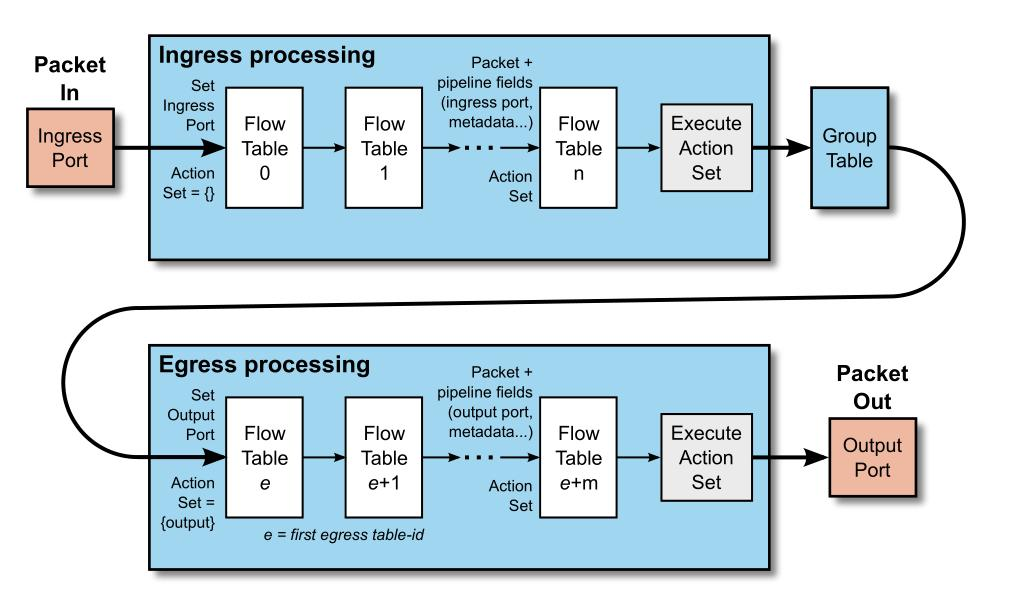
\includegraphics[scale=0.5]{imgs/pkt_flow.jpg}
	\caption{نمایی از جریان پردازش بسته‌ها در خط لوله}
	\label{fig5}
\end{figure}

پس از ورود بسته‌ها از طریق درگاه‌های معرفی شده، پردازش بر روی آن‌ها از طریق خط لوله انجام می‌گیرد. سوئیچ‌ها از لحاظ پشتیبانی \lr{Openflow} به دو دسته سوئیچ‌های \lr{Openflow-only} و \lr{Openflow-hybrid} تقسیم می‌شوند.\\
در سوئیچ‌های نوع \lr{Openflow-only} تمام بسته‌ها توسط خط لوله \lr{Openflow} پردازش شده و به خروجی تحویل داده می‌شوند اما در سوئیچ‌های نوع \lr{Openflow-hybrid} بسته‌ها می‌توانند از خط لوله \lr{Openflow} یا خط لوله \lr{non-Openflow} و یا هر دو به صورت سری پردازش شوند که نوع و ترتیب این پردازش‌ها با توجه به نوع پیکربندی و همچنین سازنده تجهیزات می‌تواند متفاوت باشد.\\
با توجه به شکل \ref{fig5} هر خط لوله از اجزاء و مراحل پردازشی جداگانه تشکیل شده است که در ادامه به توضیح مختصری در باره آن‌ها می‌پردازیم. 
\begin{itemize}
	\item \lr{Ingress Port}:
این درگاه به منظور ایجاد بستری برای ورود اطلاعات به خط لوله پردازش می‌باشد که می‌تواند از یکی از انواع درگاه فیزیکی یا درگاه منطقی باشد.

	\item \lr{Ingress Processing}:
بخش اول پردازش بسته‌ها پس از ورود به خط لوله در اینجا انجام می‌گیرد. به هر بسته ورودی یک مجموعه تهی \lr{Action-Set} نسبت داده می‌شود. این مجموعه در طی عبور بسته از جداول جریان توسط عملیات‌های مورد نیاز برای بسته پر شده و در انتهای پردازش، بخش \lr{Execute Action-Set} عملیات‌ها را به صورت دسته‌ای و به ترتیب اولویت بر روی بسته اعمال می‌کند. در ارتباط با جداول جریان\LTRfootnote{Flow Table} و مدخل‌های ورودی\LTRfootnote{Flow Entry} در بخش بعدی به طور کامل توضیح خواهیم داد.

	\item \lr{Group Table}:
یکی از عناصر مهم خط لوله پردازش می‌باشد که از نسخه‌ی \lr{OF1.1} به استاندارد اضافه شده است. این جدول امکان ایجاد عملیات‌های پیچیده و خاص را بر روی بسته‌ها فراهم می‌کنید و همچنین در مواردی باعث کاهش مقدار پردازش در بخش‌های قبلی و بعدی می‌شود. در بخش‌های آینده به صورت کامل کاربرد و نحوه عملکرد این واحد را شرح خواهیم داد.

	\item \lr{Egress Processing}:
همانطور که در شکل \ref{fig5} قابل مشاهده است، این مرحله از پردازش توسط جداول جریان در مرحله آخر و قبل از ارسال بسته به خروجی قرار دارد که امکانات ویژه‌ای جهت ایجاد سناریو‌های خاص فراهم می‌آورد. این ویژگی از نسخه \lr{OF1.5} به استاندارد اضافه شده که در فصل آینده در مورد ویژگی‌ها و تفاوت‌های آن را با \lr{Ingress processing} به صورت کامل توضیح خواهیم داد.

	\item \lr{Output Port}:
این درگاه به منظور ایجاد بستری برای خروج بسته‌های پردازش شده توسط خط لوله می‌باشد که می‌تواند یکی از انواع درگاه‌های تعریف شده در استاندارد برای خروجی در نظر گرفته شود.

\end{itemize}

\subsection{\lr{Flow Tables}}
با توجه به شکل \ref{fig5} هر یک از مراحل \lr{Ingress/Egress Processing} دارای چندین جدول جریان می‌باشند. هر جدول جریان نیز دارای یک یا چند مدخل جریان است. هر مدخل جریان نیز به صورت زیر تعریف می‌گردد:
\begin{table}[ht]
	\centering
	\begin{latin}
		\begin{tabular}[t]{|c|c|c|c|c|c|c|}
			\hline
			Match Fields & Priority & Counters & Instructions & Timeouts & Cookie & Flags\\
			\hline
		\end{tabular}
	\end{latin}
	\caption{\rl{اجزاء اصلی یک مدخل جریان}}
	\label{tab1}
\end{table}

\begin{itemize}
	\item \lr{Match Fields}:
برای ایجاد تطابق با بسته‌ها کاربرد دارد که از قسمت‌های درگاه ورودی\LTRfootnote{Ingress Port}، سرآیند‌های بسته‌ها\LTRfootnote{Packet Headers} و به صورت اختیاری پارامتر‌های خط لوله\LTRfootnote{Pipeline Fields} مانند فراداده‌های\LTRfootnote{Metadata} جدول‌های پیشین تشکیل شده است.
	\item \lr{Priority}:
نشان دهنده اولویت بسته‌ها به منظور انجام تطابق می‌باشد.
	\item \lr{Counters}:
با انجام شدن عمل تطابق شمارنده‌ها افزایش می‌یابند تا داده‌های آماری مربوط به جدول جریان را کامل کنند.
	\item \lr{Instructions}:
به منظور ایجاد تغییر در مجموعه \lr{Action-Set} از این پارامتر در مدخل جریان می‌توان استفاده کرد.
	\item \lr{Timeouts}:
حداکثر زمان و مدت زمان \lr{Idle} که یک مدخل جریان پس از آن باطل می‌شود در این قسمت قابل برنامه ریزی می‌باشد.
	\item \lr{Cookie}:
این پارامتر را کنترل کننده‌ها به منظور عملیات داخلی استفاده می‌کنند.
	\item \lr{Flags}:
توسط این پارامتر‌ها می‌توان نحوه مدیریت مدخل‌های جریان را در جدول جریان تغییر داد.
\end{itemize}

باید به این نکته توجه داشت که همه کنترل کننده‌ها و همه سوئیچ‌ها قابلیت پشتیبانی از همه عملیات‌های گفته شده در بالا را ندارند که این قابلیت‌ها بسته به پیاده سازی برند‌های مختلف از پروتکل متفاوت می‌باشد.

\subsection{\lr{Table-miss}}
در هر جدول جریان، در صورتی که عمل تطابق در آن صورت نگیرد، مدخل جریانی به نام \lr{Table-miss} در آن وجود دارد که وضعیت بسته را برای ادامه در خط لوله مشخص می‌کند. برای مثال می‌توان بسته را دور انداخت یا به جدول جریان بعدی و یا به کنترل کننده ارسال کرد.\\

\begin{figure}
	\centering
	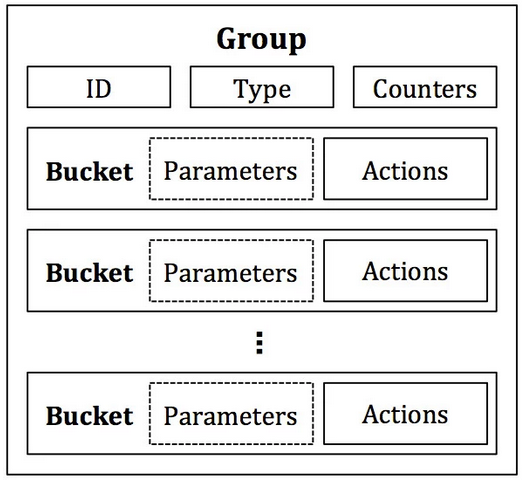
\includegraphics[scale=0.5]{imgs/group_fig.png}
	\caption{نمایی از شکل کلی جدول گروه}
	\label{fig6}
\end{figure}

\subsection{\lr{Group Table}}
همان طور که در بخش قبلی نیز بیان شد، جدول گروه، انتزاعی به منظور پیاده سازی عملیات‌های پیچیده و خاص است که قابلیت پیاده سازی آسان با استفاده از جداول جریان و مدخل‌های آن‌ها را ندارند.هر گروه در این جدول بسته‌ها را با عنوان ورودی دریافت کرده و عملیات‌های به خصوصی را روی آن‌ها انجام می‌دهند.\\
هر گروه دارای دسته‌ای از عملیات‌ها است که سطل\LTRfootnote{Bucket} نامیده می‌شوند. همان طور که در شکل \ref{fig6} مشاهده می‌شود، گروه می‌تواند نوع\LTRfootnote{Type} مختلفی داشته باشد که در ادامه به آن‌ها اشاره و کاربرد آن‌ها را بررسی می‌کنیم:

\begin{itemize}
	\item \lr{ALL}:
در این حالت، بسته‌های ورودی به صورت یکسان به تمام سطل‌ها وارد شده و سری عملیات\LTRfootnote{Actions} بخصوصی به صورت مستقل بر روی آن‌ها انجام می‌گیرد. می‌توان از این ویژگی به منظور ایجاد، پردازش و ارسال داده‌ها به صورت \lr{Broadcast} و یا \lr{Multicast} استفاده کرد.
	\item \lr{INDIRECT}:
در این گروه به خصوص فقط یک سطل وجود دارد و تمام بسته‌های ورودی به گروه به آن وارد می‌شوند. کاربرد مهم این گروه، ایجاد قابلیت جمع آوری عملیات تکراری در جداول جریان و اجراء آن‌ها در یک مرتبه به منظور کاهش سربار پردازشی و حافظه‌ای است.
	\item \lr{SELECT}:
در این گروه، سطل‌ها به صورت وزن دار اولویت برای دریافت بسته دارند. کاربرد اصلی این گروه به منظور ایجاد تراز بار\LTRfootnote{Load Balancing} در شبکه است و واضح‌ترین الگوریتم برای ایجاد توازن در این گروه \lr{Round-Robin} می‌باشد اما از الگوریتم‌های پیچیده‌تر و بهینه‌تری نیز می‌توان استفاده کرد..
\end{itemize}

\subsection{\lr{Meter Table}}
در نسخه \lr{OF1.3}، مفهومی به نام اندازه‌گیر‌ها\LTRfootnote{Meters} به استاندارد \lr{Openflow} افزوده شد. با ترکیب این اندازه‌گیر‌ها و بستر صف‌های خروجی می‌توان به صورت کلی نرخ دریافت و ارسال بسته از سوئیچ را اندازه‌گیری و کنترل کرد. جداول جریان قادر به ارسال بسته‌ها به سمت جداول اندازه‌گیر هستند که این خود زمینه ایجاد کنترل کیفیت سرویس\LTRfootnote{Quality of Service (QoS)} را فراهم می‌آورد.

\section{بررسی وظایف مهم در خط لوله}
در طول خط لوله، سه وظیفه اصلی و مهم انجام می‌گیرد که در اینجا به بررسی آن‌ها می‌پردازیم.

\subsection{\lr{Match}}
در هنگام دریافت بسته، سوئیچ توابع به خصوصی را به منظور انجام پردازش در خط لوله اجرا می‌کند. در ابتدا سوئیچ فیلد‌های بسته را به منظور جستجو و انجام عمل تطابق در جداول جریان جداسازی می‌کند. این فیلد‌ها می‌تواند شامل فیلد‌های سرآیند‌های مختلف مانند \lr{Ethernet} و یا \lr{TCP/IP} باشد. علاوه بر سرآیند‌های بسته، تطابق می‌تواند برای پورت ورودی، فراداده‌ها و دیگر فیلد‌های خط لوله نیز انجام بپذیرد. فراداده‌ها ممکن است به منظور انتقال اطلاعات بین جداول سوئیچ استفاده شود. تمام فیلد‌های سرآیند‌ها و فیلد‌های خط لوله نمایانگر وضعیت فعلی بسته هستند. در صورتی که بسته توسط جدول‌های قبلی دچار تغییر شده باشد، تطابق بر روی مقادیر جدید انجام می‌گیرد.\\
یک بسته هنگامی با یکی از مدخل‌های جریان تطابق می‌یابد که تمام فیلد‌های سرآیند و خط لوله آن مطابقت داشته باشد. در صورتی که یک بسته به چند مدخل جریان مطابقت داشت، مدخل جریانی که اولویت\LTRfootnote{Priority} بالاتری داشته باشد عملیات را روی بسته انجام خواهد داد.

\subsection{\lr{Instruction}}
هر مدخل جریان دارای یک سری از دستورات است و زمانی که بسته‌ای با آن مدخل جریان تطابق یافت، دستورات روی بسته اجرا می‌گردند. هر دستور می‌تواند در مجموعه عملیات\LTRfootnote{Action-Set} و یا در پردازش خط لوله بسته تغییر ایجاد کند. نمونه‌ای از دستورات به شرح زیر می‌باشد:
\begin{itemize}
	\item \lr{Apply-Actions}:
پیاده سازی آنی تغییرات روی بسته بدون تغییر در مجموعه عملیات بسته
	\item \lr{Clear-Actions}:
پاک کردن تمام عملیات‌های موجود در مجموعه عملیات
	\item \lr{Write-Actions}:
اضافه کردن عملیات به مجموعه عملیات بسته
	\item \lr{Write-Metadata}:
اضافه کردن فرداده به فیلد مربوطه در بسته
	\item \lr{Stat-Trigger}:
درصورتی که آمار مرتبط با یکی از جریان‌ها به حدود تعریف شده رسیده باشد به کنترل کننده یک رخداد ارسال می‌کند.
	\item \lr{Goto-Table}:
نشان دهنده جدول بعدی به منظور ادامه پردازش خط لوله می‌باشد.
\end{itemize}
\subsubsection{\lr{Action}}
همان طور که در بالا اشاره شد، هر دستور یک عملیات روی بسته انجام می‌دهد یا یک عملیات در مجموعه عملیات بسته وارد می‌کند. از مجموعه عملیات‌های ممکن روی بسته می‌توان به موارد زیر اشاره کرد:
\begin{itemize}
	\item \lr{Output \textit{port\_no}}:
باعث هدایت بسته به درگاه مورد نظر به منظور انجام پردازش خروجی و خارج شدن بسته از سوئیچ می‌باشد.
	\item \lr{Group \textit{group\_id}}:
مشخص کردن گروه به منظور هدایت بسته به آن و انجام پردازش‌های مرتبط با گروه.
	\item \lr{Drop}:
بسته‌هایی که هیچ گونه عملیات مشخصی برای انجام نداشته باشند درنهایت رها می‌شوند.
	\item \lr{Set-Queue \textit{queue\_id}}:
به منظور مشخص کردن صف خروجی بسته می‌باشد.
	\item \lr{Meter \textit{meter\_no}}:
بسته‌هایی که باید به سمت اندازه‌گیر‌ها هدایت شوند توسط این عملیات مشخص می‌گردند.
	\item \lr{Push-Tag/Pop-Tag \textit{ethertype}}:
به منظور تغییر نوع بسته بکار می‌رود. برای مثال می‌توان نوع سرآیند بسته را برای پیاده سازی \lr{MPLS} تغییر داد.
	\item \lr{Set-Field \textit{field\_type value}}:
توسط این عملیات می‌توان فیلد‌های مختلف موجود در سرآیند بسته‌ها را تغییر داد.
	\item \lr{Copy-Field \textit{src\_field\_type dst\_field\_type}}:
توسط این عملیات می‌توان فیلد‌های مختلف موجود در سرآیند یک بسته را به سرآیند بسته دیگر رونوشت کرد.
	\item \lr{Change-TTL \textit{ttl}}:
توسط این عملیات می‌توان مقدار \lr{TTL} بسته را ویرایش کرد.
\end{itemize}

\subsection{\lr{Counter}}
شمارنده‌ها برای هر جدول جریان، مدخل جریان، درگاه، صف، گروه، سطل گروه و اندازه‌گیر وجود دارند. در هر بخش، شمارنده‌ها، مولفه‌های مرتبط با آن بخش را شمارش کرده و به صورت داده‌های آماری به کنترل کننده ارسال می‌کنند. تمامی شمارنده‌های موجود به صورت بدون علامت بوده و نمایشگر سرریز\LTRfootnote{OverFlow} ندارند. نمونه‌هایی از شمارنده‌های موجود برای یک مدخل جریان عبارت‌اند از: تعداد بسته‌های دریافت شده، تعداد بایت‌‌های دریافت شده، مدت زمان وجود مدخل بر حسب ثانیه.
